\documentclass[9pt,hyperref={pdfpagelabels=false},xcolor=table]{beamer}
\usepackage{multicol}

% Contact information: 
%   Jorge M. Cruz-Duarte (jorge.cruz@tec.mx)
%   Nov. 29, 2019

\input{tecbeamer.tex}

\title{Optimizing Gaussian Processes}  
\author[Michael Ciccotosto-Camp]{{\bf Honours Research Project}} 
%\institute{}
\date{
Michael Ciccotosto-Camp - 44302913 \\
}

\begin{document}

\maketitle

\section{Problem Significance}

\begin{frame}
    \frametitle{Problem Setting and Motivation}
    \begin{itemize}
        \item A survey of various parameteric models to compare with Gaussian processes.
    \end{itemize}
    \begin{figure}
        \centering
        \includegraphics[scale=0.18]{img/yan_wheat_GPR_plot.png}
    \end{figure}
\end{frame}

\begin{frame}
    \begin{itemize}
        \item Photo courtesy of A/Prof Andries Potgieter and Dr Yan Zhao.
    \end{itemize}
    \begin{figure}
        \centering
        \includegraphics[scale=0.51]{img/yan_crop_id.png}
    \end{figure}
\end{frame}

\begin{frame}
    \begin{figure}
        \centering
        \subfloat[]{
            \begin{adjustbox}{width=0.5\textwidth}
                \includegraphics[scale=0.5]{img/vital_signs.PNG}
            \end{adjustbox}
        }
        \subfloat[]{
            \begin{adjustbox}{width=0.5\textwidth}
                \includegraphics[scale=0.5]{img/robot_damaged.PNG}
            \end{adjustbox}
        }
    \end{figure}
    \begin{itemize}
        \item (A) Gaussian processes used to filter noise from medical data, photo courtesy of R. Durichen etal. (B) Gaussian processes used to help robots adapt to physical impairments, photo courtesy of A. Cully etal.
    \end{itemize}
\end{frame}

\section{Gaussian Processes}

\begin{frame}
    \frametitle{Introduction to Gaussian Processes}
    \begin{itemize}
        \item Gaussian Process (GP) are completely characterized by a mean function $m : X \to \mathbb{R}$ and a kernel $k : X \times X \to \mathbb{R}$.
    \end{itemize}
    \begin{align*}
        m(\bm{x})           & = \mathbb{E} \left[ f(\bm{x}) \right]                                          \\
        k (\bm{x}, \bm{x'}) & = \mathbb{E} \left[ (f(\bm{x}) - m(\bm{x})) (f(\bm{x'}) - m(\bm{x'})) \right].
    \end{align*}
\end{frame}

\begin{frame}
    \begin{itemize}
        \item A very common kernel function used is the RBF or Gaussian kernel.
    \end{itemize}
    \vspace*{-\baselineskip}
    \vspace*{-\baselineskip}
    \begin{figure}[h]
        \centering
        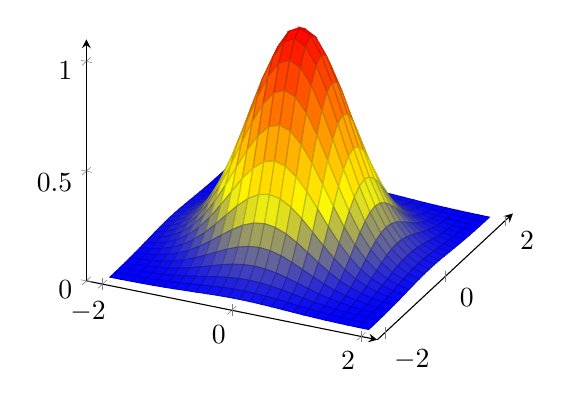
\begin{tikzpicture}

            \begin{axis}[
                    width=7cm,height=7cm,
                    domain=-2:2,
                    xmax=2.25,
                    ymax=2.25,
                    xmin=-2.25,
                    ymin=-2.25,
                    zmax=1.1,
                    axis lines = left,
                    colormap/hot,
                ]

                \addplot3[samples = 25, surf] {exp(-(x^2 + y^2)/1)};

            \end{axis}

        \end{tikzpicture}
    \end{figure}
\end{frame}

\begin{frame}
    \frametitle{Predictions}
    \begin{itemize}
        \item Our data and novel points should form a joint Gaussian distribution
              \[
                  \begin{bmatrix}
                      \bm{y} \\
                      \bm{y}_{\star}
                  \end{bmatrix}
                  \sim \mathcal{N}
                  \begin{pmatrix}
                      \bm{0}, &
                      {
                              \begin{bmatrix}
                                  \bm{K_{XX}} + \sigma_n^2 \mathbb{I}_{n \times n} & \bm{K_{X_{\star}X}^{\intercal}} \\
                                  \bm{K_{X_{\star}X}}                              & \bm{K_{X_{\star}X_{\star}}}
                              \end{bmatrix}
                          }
                  \end{pmatrix}.
              \]
              (using the notation $\left( \bm{K}_{\bm{W} \bm{W}'} \right)_{i,j} \triangleq k \left( \bm{w}_i , \bm{w}_j' \right)$)
              \pause
        \item The mean and covariance can then be computed as
              \begin{align*}
                  \overline{\bm{y}_{\star}}           & = \bm{K_{X_{\star}X}} \left[ \bm{K_{XX}} + \sigma_n^2 \mathbb{I}_{n \times n} \right]^{-1} \bm{y}                                                         \\
                  \operatorname{cov} (\bm{y}_{\star}) & = \bm{K_{X_{\star}X_{\star}}} - \bm{K_{X_{\star}X}} \left[ \bm{K_{XX}} + \sigma_n^2 \mathbb{I}_{n \times n} \right]^{-1} \bm{K_{X_{\star}X}}^{\intercal}.
              \end{align*}
    \end{itemize}
\end{frame}

\begin{frame}
    \frametitle{Unoptimized GPR}
    {\centering
        \begin{minipage}{.9\linewidth}
            \begin{algorithm}[H]
                \caption{Unoptimized GPR}
                \SetAlgoLined
                \DontPrintSemicolon
                \SetKwInOut{Input}{input}\SetKwInOut{Output}{output}

                \Input{Observations $\bm{X}, \bm{y}$ and a test input $\bm{x}_{\star}$.}
                \Output{A prediction $\overline{y_{\star}} $ with its corresponding variance $ \mathbb{V} \left[ y_{\star} \right]$.}
                \BlankLine
                $\bm{L} = \operatorname{cholesky} \left( \bm{K_{XX}} + \sigma_n^2 \mathbb{I}_{n \times n} \right)$\;
                $\bm{\alpha} = \operatorname{lin-solve} \left( \bm{L}^{\intercal} , \operatorname{lin-solve} \left( \bm{L}, \bm{y} \right) \right)$\;
                $\overline{y_{\star}} = \bm{K_{x_{\star} X}} \bm{\alpha}$\;
                $\bm{v} = \operatorname{lin-solve} \left( \bm{L}, \bm{K_{x_{\star} X}} \right)$\;
                $\mathbb{V} \left[ y_{\star} \right] = \bm{K_{x_{\star} x_{\star}}} - \bm{v}^{\intercal} \bm{v}$\;
                \Return{$\overline{y_{\star}} , \mathbb{V} \left[ y_{\star} \right]$}
                \BlankLine
            \end{algorithm}
        \end{minipage}
        \par
    }
\end{frame}

\begin{frame}[fragile]
    \frametitle{Implementation}

    \begin{minted}{python}
    def gp_reg_pred(X_train, Y_train, x_pred, sigma):
        n, d = X_train.shape
        # Create the Gram matrix corresponding to the training data set.
        K = exact_kernel(X_train, sigma=sigma)
        # Noise variance of labels.
        s = np.var(Y_train.squeeze())
        L = np.linalg.cholesky(K + s*np.eye(n))
        # Compute the mean at our test points.
        Lk = np.linalg.solve(L, exact_kernel(X_train, x_pred, sigma=sigma))
        Ef = np.dot(Lk.T, np.linalg.solve(L, Y_train))
        # Compute the variance at our test points.
        K_ = exact_kernel(x_pred, sigma=sigma)
        Vf = np.diag(K_) - np.sum(Lk**2, axis=0)
        return Ef, Vf
    \end{minted}

\end{frame}

\begin{frame}
    \frametitle{Stock Market Prediction}

    \begin{figure}
        \centering
        \begin{adjustbox}{width=0.9\textwidth}
            \includegraphics[scale=1]{img/stock_eg.png}
        \end{adjustbox}
    \end{figure}
\end{frame}

\begin{frame}
    \frametitle{Problems with Unoptimized GPR}
    {\centering
        \begin{minipage}{.9\linewidth}
            \begin{algorithm}[H]
                \caption{Unoptimized GPR}
                \SetAlgoLined
                \DontPrintSemicolon
                \SetKwInOut{Input}{input}\SetKwInOut{Output}{output}

                \Input{Observations $\bm{X}, \bm{y}$ and a prediction inputs $\bm{x}_{\star}$.}
                \Output{A prediction $\overline{y_{\star}} $ with its corresponding variance $ \mathbb{V} \left[ y_{\star} \right]$.}
                \BlankLine
                \textcolor{red}{$\bm{L} = \operatorname{cholesky} \left( \bm{K_{XX}} + \sigma_n^2 \mathbb{I}_{n \times n} \right)$}\;
                \textcolor{red}{$\bm{\alpha} = \operatorname{lin-solve} \left( \bm{L}^{\intercal} , \operatorname{lin-solve} \left( \bm{L}, \bm{y} \right) \right)$}\;
                $\overline{y_{\star}} = \bm{K_{x_{\star} X}} \bm{\alpha}$\;
                \textcolor{red}{$\bm{v} = \operatorname{lin-solve} \left( \bm{L}, \bm{K_{x_{\star} X}} \right)$}\;
                $\mathbb{V} \left[ y_{\star} \right] = \bm{K_{x_{\star} x_{\star}}} - \bm{v}^{\intercal} \bm{v}$\;
                \Return{$\overline{y_{\star}} , \mathbb{V} \left[ y_{\star} \right]$}
                \BlankLine
            \end{algorithm}
        \end{minipage}
        \par
    }
\end{frame}

\begin{frame}
    \begin{itemize}
        \item The bottle necks that we would like to address are the computation of \textcolor{red}{$\bm{K_{X X}}$} and the \textcolor{red}{Cholesky} decomposition.
              \pause
              \bigskip
        \item Exact computation of \textcolor{red}{$\bm{K_{X X}}$} replaced with \textcolor{blue}{Nystrom} and \textcolor{blue}{RFF} estimates.
              \pause
              \bigskip
        \item Looked at \textcolor{blue}{CG} and \textcolor{blue}{MINRES} to replace \textcolor{red}{Cholesky} decomposition.
    \end{itemize}
\end{frame}

\section{Nystrom}

\begin{frame}
    \frametitle{Nystrom Approximation}
    \begin{itemize}
        \item The Nystrom method we seek a matrix $\bm{Q}\in \mathbb{R}^{n \times k}$ that satisfies $\norm{\bm{A} - \bm{Q} \bm{Q}^{\ast} \bm{A}}_{F} \leq \varepsilon$, where $\bm{A} \in \mathbb{R}^{n \times n}$ is positive semi definite matrix, to form the rank$-k$ approximation
              \begin{align*}
                  \onslide<1->{}
                  \onslide<2->{\bm{A} & \simeq \bm{Q} \bm{Q}^{\ast} \bm{A}                                                                                                                                \\}
                  \onslide<3->{       & \simeq \bm{Q} \left( \bm{Q}^{\ast} \bm{A} \bm{Q} \right) \bm{Q}^{\ast}                                                                                            \\}
                  \onslide<4->{       & = \bm{Q} \left( \bm{Q}^{\ast} \bm{A} \bm{Q} \right) \left( \bm{Q}^{\ast} \bm{A} \bm{Q} \right)^{\dagger} \left( \bm{Q}^{\ast} \bm{A} \bm{Q} \right) \bm{Q}^{\ast} \\}
                  \onslide<5->{       & \simeq \left( \bm{A} \bm{Q} \right) \left( \bm{Q}^{\ast} \bm{A} \bm{Q} \right)^{\dagger} \left( \bm{Q}^{\ast} \bm{A} \right).}
              \end{align*}
              % \item This tells us that $\bm{K_{XX}}$ can be computed as $\bm{K_{XX}} \simeq \bm{K}_{(:,I)} \bm{K}_{(I,I)} \bm{K}_{(:,I)}^{\intercal}$ (up to a rescaling of entries) where $I$ is a randomly sampled subset of column indices.
    \end{itemize}
\end{frame}

\section{Random Fourier Features}

\begin{frame}
    \frametitle{Random Fourier Feature Approximation}
    \begin{itemize}
        \item The RFF technique hinges on Bochners theorem which characterises positive definite functions (namely kernels) and states that any positive definite functions can be represented as
              \[
                  k \left( \bm{x}, \bm{y} \right) = k \left( \bm{x} - \bm{y} \right) = \int_{\mathbb{C}^d} \exp \left( i \langle \bm{\omega} , \bm{x} - \bm{y} \rangle \right) \mu_k \left( d \bm{\omega} \right)
              \]
              where $\mu_k$ is a positive finite measure on the frequencies of $\bm{\omega}$.
              \pause
        \item This integral can then be approximated via the following Monte Carlo estimate
              \begin{align*}
                  \onslide<1->{}
                  \onslide<2->{k \left( \bm{x} - \bm{y} \right)
                                & = \int_{\mathbb{C}^d} \exp \left( i \langle \bm{\omega} , \bm{x} - \bm{y} \rangle \right) p (\bm{\omega}) \; d \bm{\omega}                                                                                                     \\}
                  \onslide<3->{ & = \mathbb{E}_{\bm{\omega} \sim p (\cdot)} \left( \exp \left( i \langle \bm{\omega} , \bm{x} - \bm{y} \rangle \right) \right)                                                                                                   \\}
                  \onslide<4->{ & \simeq \frac{1}{D} \sum_{j=1}^{D} \exp \left( i \langle \bm{\omega}_{j} , \bm{x} - \bm{y} \rangle \right)                                                                                                                      \\}
                  \onslide<5->{ & = \sum_{j=1}^{D} \left( \frac{1}{\sqrt{D}} \exp \left( i \langle \bm{\omega}_{j} , \bm{x} \rangle \right) \right) \overline{\left( \frac{1}{\sqrt{D}} \exp \left( i \langle \bm{\omega}_{j} , \bm{y} \rangle \right) \right) } \\}
                  \onslide<6->{ & = \langle \varphi (\bm{x}) , \varphi (\bm{y}) \rangle_{\mathbb{C}^D}}
              \end{align*}
    \end{itemize}
\end{frame}

\section{Krylov Subspace Methods}

\begin{frame}
    \frametitle{Krylov Subspace Methods}
    \begin{itemize}
        \item $\bm{A} \bm{x^{\star}} = \bm{b}$.
              \pause
              \bigskip
        \item $\bm{x^{\star}} \in \bm{x}_0 + \mathcal{K}_{n} \left( \bm{A},\bm{v} \right)$ where  $\mathcal{K}_{k} \left( \bm{A},\bm{v} \right) = \operatorname{l.s} \left\{ \bm{r}_0, \bm{A} \bm{r}_0, \bm{A}^2 \bm{r}_0, \ldots , \bm{A}^{k-1} \bm{r}_0 \right\}$.
              \pause
              \bigskip
        \item CG: $\| \bm{x} - \bm{x}^{\star} \|_{\bm{A}}$ is minimized.
              \pause
              \bigskip
        \item MINRES: $\norm{\bm{A} \bm {x} - \bm{b}}_2$ is minimized.
    \end{itemize}
\end{frame}

\section{Results}

\begin{frame}
    \begin{figure}
        \centering
        \includegraphics[scale=0.4]{img/results/nys-sigma=0.1-k=80.png}
        \caption{3D-Spatial Network dataset using Nystrom}
    \end{figure}
\end{frame}

\begin{frame}
    \begin{figure}
        \centering
        \includegraphics[scale=0.4]{img/results/nys-sigma=1.0-k=20.png}
        \caption{Abalone dataset using Nystrom}
    \end{figure}
\end{frame}

\begin{frame}
    \begin{figure}
        \centering
        \includegraphics[scale=0.4]{img/results/nys-sigma=1.0-k=80.png}
        \caption{Temperature dataset using Nystrom}
    \end{figure}
\end{frame}

\begin{frame}
    \begin{figure}
        \centering
        \includegraphics[scale=0.4]{img/results/rff-sigma=0.1.png}
        \caption{3D-Spatial Network dataset using RFF}
    \end{figure}
\end{frame}

% \begin{frame}
%     \begin{figure}
%         \centering
%         \subfloat[3D-Spatial Network]{
%             \begin{adjustbox}{width=0.31\textwidth}
%                 \includegraphics[scale=1]{img/results/nys-sigma=0.1-k=80.png}
%             \end{adjustbox}
%         }
%         \subfloat[Abalone]{
%             \begin{adjustbox}{width=0.31\textwidth}
%                 \includegraphics[scale=1]{img/results/nys-sigma=1.0-k=20.png}
%             \end{adjustbox}
%         }
%         \subfloat[Temperature]{
%             \begin{adjustbox}{width=0.31\textwidth}
%                 \includegraphics[scale=1]{img/results/nys-sigma=1.0-k=80.png}
%             \end{adjustbox}
%         }
%         \caption{Comparison of Nystrom methods for various datasets.}
%     \end{figure}
%     \begin{figure}
%         \centering
%         \subfloat[3D-Spatial network]{
%             \begin{adjustbox}{width=0.31\textwidth}
%                 \includegraphics[scale=1]{img/results/rff-sigma=0.1.png}
%             \end{adjustbox}
%         }
%         \subfloat[Abalone]{
%             \begin{adjustbox}{width=0.31\textwidth}
%                 \includegraphics[scale=1]{img/results/rff-sigma=10.0.png}
%             \end{adjustbox}
%         }
%         \subfloat[Wine]{
%             \begin{adjustbox}{width=0.31\textwidth}
%                 \includegraphics[scale=1]{img/results/rff-sigma=2.1.png}
%             \end{adjustbox}
%         }
%         \caption{Comparison of RFF methods for various datasets.}
%     \end{figure}
% \end{frame}

\begin{frame}
    \begin{figure}
        \centering
        \subfloat[Frobenius error]{
            \begin{adjustbox}{width=0.45\textwidth}
                \includegraphics[scale=1]{img/results/cmp_rel-sigma=0.1-k=80.png}
            \end{adjustbox}
        }
        \subfloat[Infinity error]{
            \begin{adjustbox}{width=0.45\textwidth}
                \includegraphics[scale=1]{img/results/cmp_inf-sigma=0.1-k=80.png}
            \end{adjustbox}
        }
        \caption{Comparison between Nystrom and RFF approximations for the 3D-Spatial network data.}
    \end{figure}
\end{frame}

\begin{frame}
    \begin{itemize}
        \item How do Nystrom and RFF methods compare in terms of prediction?
    \end{itemize}
    \pause
    \begin{figure}
        \centering
        \subfloat[Stock Market dataset]{
            \begin{adjustbox}{width=0.45\textwidth}
                \includegraphics[scale=1]{img/pred/stock_market/pred_acc/kern_cmp-sigma=10.0.png}
            \end{adjustbox}
        }
        \subfloat[Temperature dataset]{
            \begin{adjustbox}{width=0.45\textwidth}
                \includegraphics[scale=1]{img/pred/temperature_data/pred_acc/kern_cmp-sigma=10.0.png}
            \end{adjustbox}
        }
        \caption{Comparison between Nystrom and RFF approximations in GP prediction.}
    \end{figure}
\end{frame}

\begin{frame}
    \begin{itemize}
        \item How do MINRES and CG methods compare in terms of prediction?
    \end{itemize}
    \begin{figure}
        \centering
        \subfloat[Abalone dataset]{
            \begin{adjustbox}{width=0.45\textwidth}
                \includegraphics[scale=1]{img/pred/abalone/pred_acc/lin_cmp-sigma=1.0.png}
            \end{adjustbox}
        }
        \subfloat[Quadratic dataset]{
            \begin{adjustbox}{width=0.45\textwidth}
                \includegraphics[scale=1]{img/pred/rastrigin/pred_acc/lin_cmp-sigma=2.1.png}
            \end{adjustbox}
        }
        \caption{Comparison between MINRES and CG in GP prediction.}
    \end{figure}
\end{frame}

\begin{frame}
    \begin{itemize}
        \item Using approximation techniques together.
    \end{itemize}
    \begin{figure}
        \centering
        \subfloat[Stock Market dataset]{
            \begin{adjustbox}{width=0.45\textwidth}
                \includegraphics[scale=1]{img/pred/3D_spatial_network/pred_acc/dual_cmp_both-sigma=1.0.png}
            \end{adjustbox}
        }
        \subfloat[Abalone dataset]{
            \begin{adjustbox}{width=0.45\textwidth}
                \includegraphics[scale=1]{img/pred/abalone/pred_acc/dual_cmp_both-sigma=1.0.png}
            \end{adjustbox}
        }
        \caption{Comparison between CG and MINRES when paried with RFF.}
    \end{figure}
\end{frame}

\begin{frame}
    \begin{itemize}
        \item $\norm{\bm{K_{X_{\star} X}} \bm{\rho} - \bm{y}_{\star}}_2^2$, where $\bm{\rho}$ is our best estimate for $\left[ \bm{K_{XX}} + \sigma_n^2 \bm{1}_{n \times n} \right] \bm{\rho} = \bm{y}$
              \bigskip
              \bigskip
              \pause
        \item $\norm{\left[ \bm{K_{XX}} + \sigma_n^2 \bm{1}_{n \times n} \right] \bm{\rho} - \bm{y}}_2^2$
    \end{itemize}
\end{frame}

\section{Moving Forward}

\begin{frame}
    \frametitle{Moving Forward}
    \begin{itemize}
        \item Write these results up.
              \bigskip
        \item Apply our findings to our initial remote sensing task.
              \bigskip
        \item Look at multi-output Gaussian Processes for remote sensing.
    \end{itemize}
\end{frame}

\begin{frame}
    \begin{figure}
        \centering
        \includegraphics[scale=0.51]{img/yan_crop_id.png}
    \end{figure}
\end{frame}

\end{document}